% Preamble of the document.
% Make this document double column.
\documentclass[6pt,twocolumn]{article}
% The secsty package provides a set of commands for changing the font
% used for the various sectional headings in the standard LATEX
\usepackage{sectsty}
% The graphicx package provides a set of commands to embed graph into the
% document.
\usepackage{graphicx}
\allsectionsfont{\sffamily\underline}

% Beginning of the document.
\begin{document}
% Title of the document.
\title{Effectiveness of Compiler Optimizations on High Level Synthesis Benchmarks}
% Author of the document.
\author{Xin Tong, University of Toronto}

% Anchor the title.
\maketitle
In general,  standard benchmarks are critically important for researchers to quantitatively measure and compare their new ideas and algorithms. CHStone is a suite of benchmark programs specifically designed for C-based high-level synthesis. It is more complex than some of the synthetic high level synthesis micro-benchmarks and yet it is self-contained and does not make use of complex data structures and functions that are difficult or impossible to synthesize onto hardware [1].
Due to the fact that researchers would like the synthesized program to run as fast as possible. Compiler level optimizations are one of the most essential stages to achieve this target. In this paper, I will investigate the effectiveness of compiler optimizations on these high level synthesis benchmarks.


% Make a section
\section{\fontsize{8}{4}\selectfont INTRODUCTION}
% Add a subsection 
\subsection{\fontsize{8}{4}\selectfont INTRODUCTION SUB}

% Skip Skip Skip 
\smallskip 
\medskip

% New page
\newpage


\begin{table}[ht]
\caption{GIVE ME A TITLE} % title of Table
\centering % used for centering table
\begin{tabular}{c c c c} % centered columns (3 columns)
\hline\hline %inserts double horizontal lines
Size & CPU2GPU & GPUEXEC & GPU2CPU \\ [0.5ex] % inserts table
%heading
\hline % inserts single horizontal line
1 &   &  &  \\
2 &   &  &  \\
3 &   &  &  \\
\hline %inserts single line
\end{tabular}
\label{table:nonlin} % is used to refer this table in the text
\end{table}

% Add some items
\begin{itemize}
\renewcommand{\labelitemi}{$\bullet$}
\item abc
\end{itemize}

% Add some arrows.
$A \rightarrow B \rightarrow C \rightarrow E,  A \rightarrow B \rightarrow D \rightarrow E \rightarrow F$.

% Make another section
\section{\fontsize{8}{4}\selectfont SECTION B}

% Embed some code.
\begin{tiny} \begin{verbatim}
 ADD CODE HERE !!!  ADD CODE HERE !!!
\end{verbatim} \end{tiny}

% Include a graph. graph can be generate with barGenerator.pl
\begin{figure}
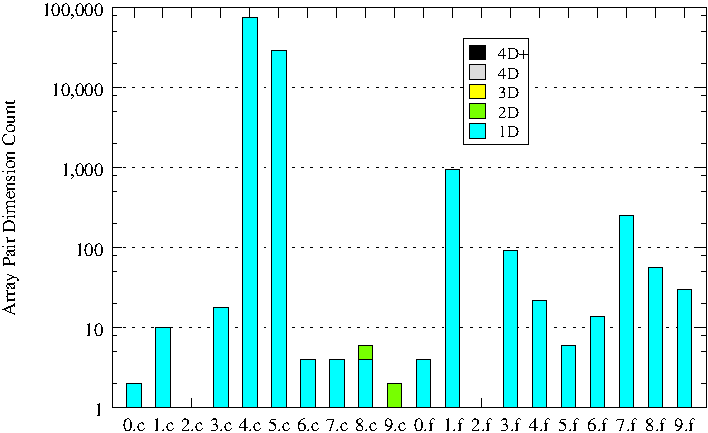
\includegraphics[width=75mm]{sample}
\caption{Sample Graph}
\end{figure}


%Add some references
% The bibliography should be embedded for final submission.
\bibliographystyle{unsrt}	% (uses file "plain.bst")
\nocite{*}
\bibliography{reference}


% End of document.
\end{document} 
